% !TeX TS-program = xelatex -synctex=1 -interaction=nonstopmode -shell-escape -output-directory=build %.tex
\documentclass[aspectratio=169]{beamer}

% All my packages are specified and set up in include/format:
\usepackage{include/format}

\title{IoT Crashcourse for Begyndere}
\subtitle{Med ESP32}

\author{Jacob Bechmann Pedersen}
\institute{Bechmann Engineering ApS}
\date{\today}

%% Reference settings:
\renewcommand{\figurename}{Figur}
\renewcommand{\tablename}{Tabel}
\renewcommand{\refname}{Referenceliste}
\renewcommand{\contentsname}{Indhold}
\renewcommand{\listfigurename}{Figurliste}
\renewcommand{\listtablename}{Tabelliste}
\renewcommand{\lstlistlistingname}{Kodeliste}

\begin{document}

\begin{frame}
	\titlepage
\end{frame}

\begin{frame}{Indhold}
	\begin{columns}
	\begin{column}{0.6\textwidth}
		\begin{fitBox}
			\tableofcontents{}
		\end{fitBox}
	\end{column}
	\begin{column}{0.4\textwidth}
		\centering
		\begin{figure}
  			\includesvg[height=0.6\textheight]{assets/svg/ESP32-DevkitC-v4.svg}
  			\caption{ESP32 DevkitC v4, boardet vi skal arbejde med}
  			\label{fig:esp32}
		\end{figure}
	\end{column}
	\end{columns}	
\end{frame}

\section{Hvem er jeg?}
\begin{frame}[fragile]{Hvem er jeg?}
\begin{columns}
	\begin{column}{0.4\textwidth}
		\begin{center}
		\roundedGfx{0.8\textwidth}{assets/pictures/portrait.png}
		\vspace{0.05\textwidth}
		\begin{columns}
			\begin{column}{0.33\textwidth}
	  			\roundedGfx{\textwidth}{assets/pictures/shiny-hunter.jpg}
			\end{column}
			\begin{column}{0.33\textwidth}
	  			\roundedGfx{\textwidth}{assets/pictures/hackrf.jpg}
			\end{column}
			\begin{column}{0.33\textwidth}
  				\roundedGfx{\textwidth}{assets/pictures/wifi-picture.jpg}
			\end{column}
		\end{columns}
		\end{center}
	\end{column}	

	\begin{column}{0.6\textwidth}
	\begin{textBox}
		Jacob Bechmann Pedersen
			\begin{itemize}
				\item Kursus-/Foredragsholder om embedded elektronik, programmering og Arduino
				\item Tidl. Embedded electronics engineer hos DTU Elektro, Automation and Control
					\begin{itemize}
						\item Robotter, embedded Linux, autonome systemer
					\end{itemize}
				\item Tidl. Embedded software developer hos Oticon
					\begin{itemize}
						\item Applikationer til høreapparaternes OS, unit- og device testing
					\end{itemize}
				\item Underviser på MakerCamp
					\begin{itemize}
						\item "Inventors" linje - 12-16 årige
					\end{itemize}
				\item Frivillig i Coding Pirates 2016-2018
				\item Electronic Design Engineer (AU, 2019)
				\item Startede med Arduino i 2014
			\end{itemize}
	\end{textBox}
	\end{column}
\end{columns}	
\end{frame}

\section{Formål}
\begin{frame}{Formål}
	\begin{textBox}
		\begin{itemize}
			\item At forstå grundprincipperne bag IoT
			\begin{itemize}
				\item Topologier
				\item Protokoller, herunder:
				\begin{itemize}
					\item HTTP
					\item Websockets
					\item MQTT
				\end{itemize}
			\end{itemize}
			\item Programmere simple implementationer
			\begin{itemize}
				\item På ESP32
				\item Med Arduino platformen
			\end{itemize}
		\end{itemize}
	\end{textBox}
\end{frame}

\section{Ressourcer}
\begin{frame}{Ressourcer}
	\begin{textBox}
	Nogle nyttige links:
		\begin{itemize}
			\item \url{https://github.com/iakop/IoT-Crashcourse}
			\begin{itemize}
				\item Præsentation og kode til denne workshop
			\end{itemize}
			\item \url{https://www.arduino.cc/en/software\#legacy-ide-18x}
			\begin{itemize}
				\item Download af Arduino IDE 1.8.X
				\item Windows version at downloade: \tthigh{Win 7 or newer}
				\item Mac OS X version at downloade: \tthigh{10.10 or newer} 
				\item Linux version at downloade: \tthigh{64 bits/Det ved du selv}\color{arduinoBlue}😜%\emojifont{😜}
			\end{itemize}
			\item \url{https://www.arduino.cc/en/reference}
			\begin{itemize}
				\item Reference for keywords i Arduino
			\end{itemize}
		\end{itemize}
	\end{textBox}
\end{frame}

\section{Dagens program}
\begin{frame}{Dagens program}
	\begin{textBox}
		\textbf{16:00 - 16:30:} Setup af ESP32 på Arduino IDE
		\begin{itemize}
			\item Board Definitions
			\item Libraries og Tools
		\end{itemize}
		\textbf{16:30 - 17:30:} Byg en simpel ESP32 webserver
		\begin{itemize}
			\item IoT basics
			\item ESP32 Webserver m. HTTP kontrol gennem webside og curl
		\end{itemize}
		\textbf{17:30 - 18:00:} Forplejning - pause\\
		\textbf{18:00 - 18:30:} Websockets på ESP32
		\begin{itemize}
			\item Udvid server med javascript og websocket forbindelse
			\item Tilføj Websocket forbindelse på ESP32
		\end{itemize}
		\textbf{18:00 - 18:30:} MQTT på ESP32
		\begin{itemize}
			\item Demo MQTT broker med flere ESP32 klienter
			\item Byg MQTT klienter til at kommunikere på fælles broker
		\end{itemize}
		\textbf{19:45 - 20:00:} Opsamling, evaluering, og afslutning
	\end{textBox}
\end{frame}

\section{Setup af ESP32 på Arduino IDE}
\begin{frame}
	\sectiontitle{assets/pictures/arduino-ide.png}{\insertsectionhead}
\end{frame}

\subsection{Board Definitions}
\begin{frame}{Board Definitions}
\begin{columns}
	\begin{column}{0.5\textwidth}
		\begin{figure}
  			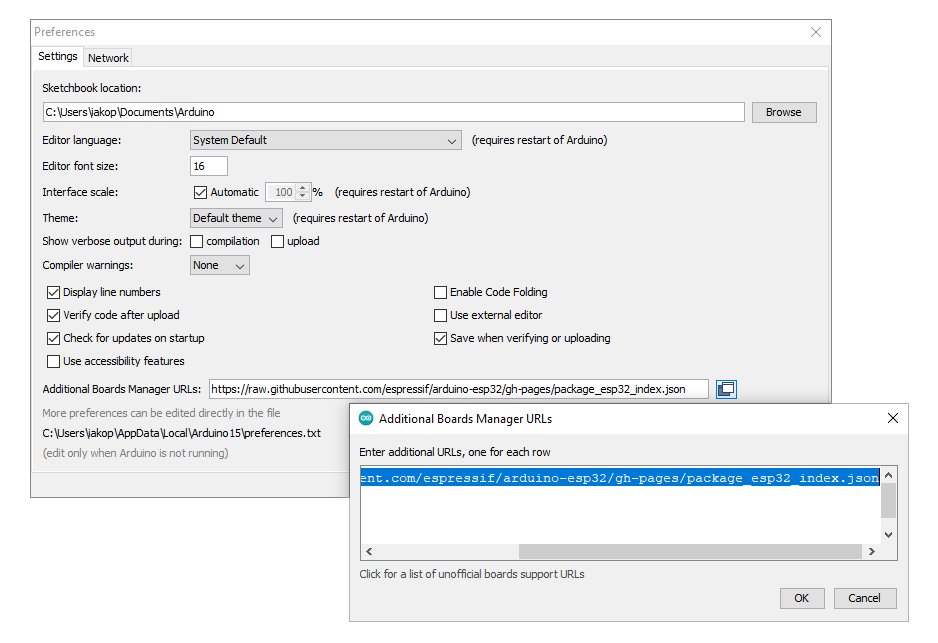
\includegraphics[width=\textwidth]{assets/pictures/boardsmanager.png}
  			\caption{Preferences manager i Arduino IDE 1.8.19}
  			\label{fig:boardmanager}
		\end{figure}
	\end{column}
	\begin{column}{0.5\textwidth}
		\begin{textBox}
			\begin{itemize}
				\item I Arduino IDE:
				\begin{itemize}
					 \item "\tthigh{File} > \tthigh{Preferences}"
				\end{itemize}
				\item Indsæt URL i "\tthigh{Additional Boards Manager URLs}":
				\begin{itemize}
					 \item \tiny\url{https://raw.githubusercontent.com/espressif/arduino-esp32/gh-pages/package_esp32_index.json}
				\end{itemize}
			\end{itemize}
		\end{textBox}
	\end{column}
\end{columns}
\end{frame}

\begin{frame}{Board Definitions}
\begin{columns}
	\begin{column}{0.5\textwidth}
		\begin{textBox}
			\begin{itemize}
				\item Under "\tthigh{Tools} > \tthigh{Board} > \tthigh{Boards Manager}"
				\item Søg efter "\tthigh{ESP32}" og tryk "\tthigh{Install}" ud fra den seneste version
				\begin{itemize}
					 \item Der skal hentes omkring 250MB, så det tager lidt tid
				\end{itemize}
			\end{itemize}
		\end{textBox}
	\end{column}
	\begin{column}{0.5\textwidth}
		\begin{figure}
  			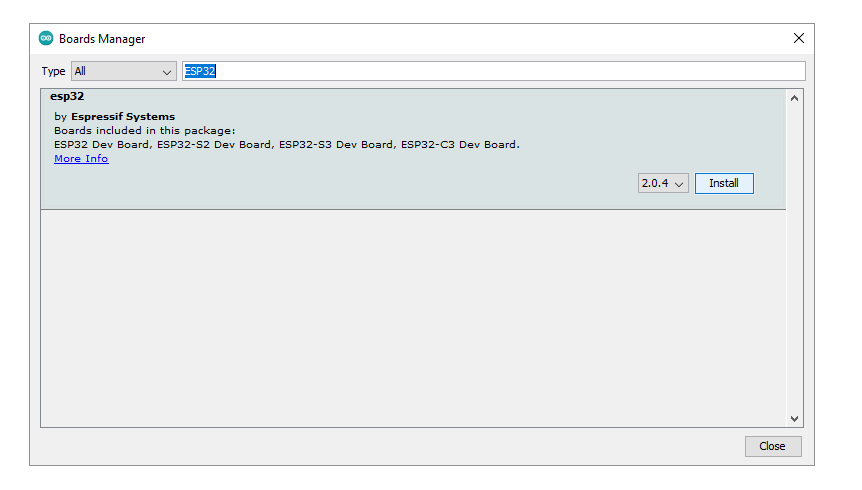
\includegraphics[width=\textwidth]{assets/pictures/boardsmanager2.png}
  			\caption{Boards Manager, her kan board definitions (beskrivelse af hardware og programmeringsværktøjer) hentes fra de kendte board manager URLs i Arduino IDE}
  			\label{fig:boardmanager2}
		\end{figure}
	\end{column}
\end{columns}
\end{frame}

\subsection{Libraries og Tools}
\begin{frame}{Libraries og Tools}
\begin{columns}
	\begin{column}{0.5\textwidth}
		\begin{figure}
			\begin{columns}
				\begin{column}{0.5\textwidth}
  					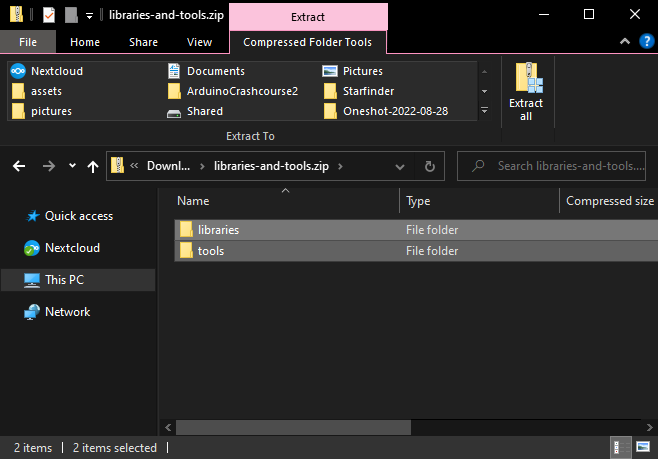
\includegraphics[width=\textwidth]{assets/pictures/libraries-and-tools-extract.png}
  				\end{column}
  				\begin{column}{0.5\textwidth}
  					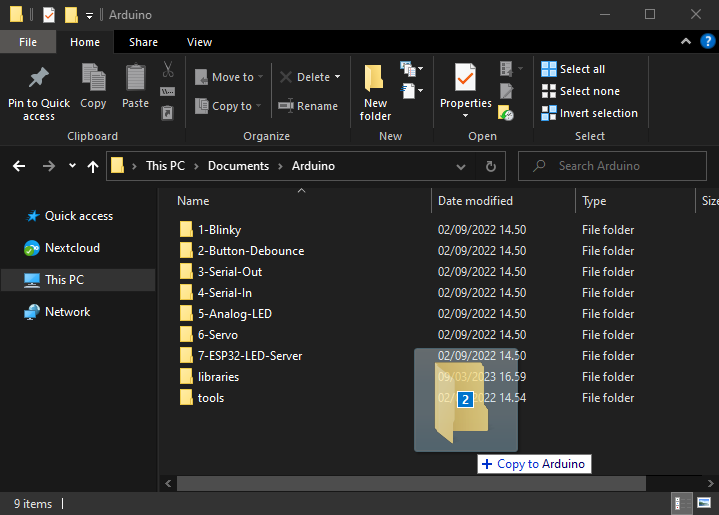
\includegraphics[width=\textwidth]{assets/pictures/copy-to-arduino.png}
  				\end{column}
  			\end{columns}
  			\caption{Arkivet indeholder to mapper, "\tthigh{libraries}" og "\tthigh{tools}" som Arduino bruger til at holde software libraries og værktøjer til IDE'et i sin default mappe under "\tthigh{Documents}/ \tthigh{Arduino}"}
  			\label{fig:libraries-and-tools}
		\end{figure}
	\end{column}
	\begin{column}{0.5\textwidth}
		\begin{textBox}
			\begin{itemize}
				\item Download arkivet "\tthigh{libraries-and-tools.zip}" fra linket:
				\begin{itemize}
					\item \tiny\url{https://raw.githubusercontent.com/iakop/IoT-Crashcourse/master/extra/libraries-and-tools.zip}
				\end{itemize}
				\item Udpak indholdet i din PC's "\tthigh{Documents}/ \tthigh{Arduino}" folder
			\end{itemize}
		\end{textBox}
	\end{column}
\end{columns}
\end{frame}

\begin{frame}{Libraries og Tools}
\begin{columns}
	\begin{column}{0.5\textwidth}
		\begin{textBox}
			\begin{itemize}
				\item For at tjekke at om de rette libraries er installeret, åbn "\tthigh{Tools} > \tthigh{Manage Libraries...}"
				\item Klik i drop-down menuen i øverste venstre hjørne på "\tthigh{Installed}"
				\item Kig her efter at pakkerne er installeret:
				\begin{itemize}
					\item \tthigh{ArduinoJson}
					\item \tthigh{DHT}
					\item \tthigh{ESPAsyncTCP}
					\item \tthigh{ESPAsyncWebSrv}
					\item \tthigh{MQTT}
				\end{itemize}
			\end{itemize}
		\end{textBox}
	\end{column}
	\begin{column}{0.5\textwidth}
		\begin{figure}
  			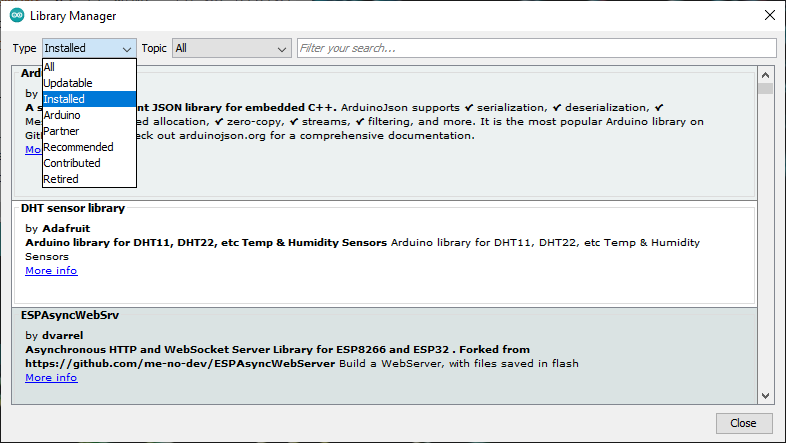
\includegraphics[width=\textwidth]{assets/pictures/librarymanager-installed.png}
  			\caption{"\tthigh{Library Manager}" kan bruges til at se de installerede libraries eller installere nye libraries der understøttes af Arduino platformen}
  			\label{fig:librarymanager-installed}
  		\end{figure}
	\end{column}
\end{columns}
\end{frame}

\begin{frame}{Libraries og Tools}
\begin{columns}
	\begin{column}{0.5\textwidth}
			\begin{figure}
  					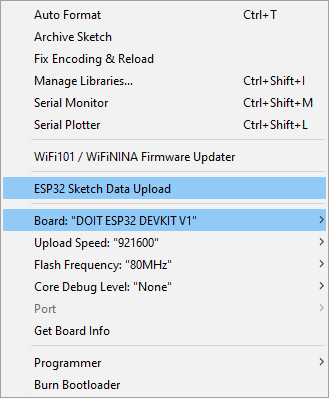
\includegraphics[width=0.5\textwidth]{assets/pictures/sketch-data-and-board.png}
  					\caption{Værktøjet "\tthigh{ESP32 Sketch Data Upload}" bruges bl.a. til at lægge .html indhold på ESP32's filsystem. Board definitionen "\tthigh{DOIT ESP32 DEVKIT V1}" sikrer, der bliver uploadet kode i det rigtige format}
  					\label{fig:sketch-data-and-board}
  			\end{figure}
	\end{column}
	\begin{column}{0.5\textwidth}
		\begin{textBox}
			\begin{itemize}
				\item For at tjekke at om de rette tools, samt Board Definitions er installeret, åbn "\tthigh{Boards}"
				\item I menuen skal feltet "\tthigh{ESP32 Sketch Data Upload}" være tilgængeligt
				\item Under feltet "\tthigh{Board:}" skal man kunne vælge "\tthigh{Board} > \tthigh{ESP32 Arduino} > \tthigh{DOIT ESP32 DEVKIT V1}"
			\end{itemize}
		\end{textBox}
	\end{column}
\end{columns}
\end{frame}

\section{IoT basics}
\begin{frame}
	\sectiontitle{assets/svg/iot-star.svg}{\insertsectionhead}
\end{frame}

\begin{frame}{IoT basics}
\begin{columns}
	\begin{column}{0.6\textwidth}
		\begin{textBox}
			\begin{itemize}
				\item IoT (Internet of Things), er en fællesbetegnelse for netværksopkoblede genstande
				\item En sådan genstand indeholder typisk:
				\begin{itemize}
					\item En microprocessor eller -computer
					\item Sensorer
					\item Aktuatorer
					\item Trådet eller trådløs opkobling
				\end{itemize}
			\end{itemize}
		\end{textBox}
	\end{column}
	\begin{column}{0.4\textwidth}
		\centering
		\begin{figure}
			\captionsetup{format=tcbcaptionminmargin}
			\roundedGfx{0.9\textwidth}{assets/pictures/nedis-smartplug.jpg}
  			\caption{Nedis SmartLife adskilt for at komme til indmaden. Indeholder bla. et TYWE3S WiFi modul og en HLW8012 effektsensor
  			\captionline \textbf{Kilde:} \url{https://callaa.github.io/2021/01/26/liberating-nedis-smartplug.html}}
  			%\caption{Nedis SmartLife adskilt for at komme til indmaden. Indeholder bla. et TYWE3S WiFi modul og en HLW8012 effektsensor}
  			\label{fig:iot-device}
		\end{figure}
	\end{column}
\end{columns}
\end{frame}

\begin{frame}{IoT basics}
\begin{columns}
	\begin{column}{0.5\textwidth}
		\centering
		\captionsetup{format=tcbcaptionsmall}
		\begin{columns}
			\begin{column}{0.5\textwidth}
				\begin{figure}[height=0.2\textheight]
  					\includesvg[height=0.2\textheight]{assets/svg/iot-star.svg}
  					\caption{Star-topologi, hvor hver enhed kommunikerer med en central gateway til resten af internettet}
  					\label{fig:iot-star}
				\end{figure}
			\end{column}
			\begin{column}{0.5\textwidth}
				\begin{figure}[height=0.2\textheight]
  					\includesvg[height=0.2\textheight]{assets/svg/iot-tree.svg}
  					\caption{Tree-topologi, hvor enhederne er forbundet i forgreninger, og videregiver informationer herigennem til gateway}
  					\label{fig:iot-tree}
				\end{figure}
			\end{column}
		\end{columns}
		\begin{columns}
			\begin{column}{0.5\textwidth}
				\begin{figure}[height=0.2\textheight]
  					\includesvg[height=0.2\textheight]{assets/svg/iot-mesh.svg}
  					\caption{Mesh-topologi, hvor alle enheder kommunikerer internt, og videre giver information gennem hinanden til gateway}
  					\label{fig:iot-mesh}
				\end{figure}
			\end{column}
		\end{columns}
	\end{column}
	\begin{column}{0.5\textwidth}
		\begin{textBox}
			\begin{itemize}
				\item Kommunikation mellem enheder foregår på mange forskellige måder
				\item Nogle gængse netværkstopologier er bla.:
				\begin{itemize}
					\item Star
					\item Tree
					\item Mesh
				\end{itemize}
			\end{itemize}
		\end{textBox}
	\end{column}
\end{columns}
\end{frame}

\begin{frame}{IoT basics}
\begin{columns}
	\begin{column}{0.6\textwidth}
		\begin{textBox}
			\begin{itemize}
				\item Der findes en række protokoller for enheder at kommunikere gennem
				\item Dem vi vil fokusere på:
				\begin{itemize}
					\item HTTP
						\begin{itemize}
							\item Den gængse Hypertext Transfer Protocol, der bruges til at overføre webindhold, bla. mellem servere og browsere
						\end{itemize}
					\item WebSocket
						\begin{itemize}
							\item En fuld duplex (tovejs kommunikation) protokol til hurtig samtidig kommunikation mellem klient og server - lav overhead
						\end{itemize}
					\item MQTT
						\begin{itemize}
							\item (Oprindeligt forkortelse for MQ (Message Queue) Telemetry Transport) Publish-subscribe baseret protokol mellem enheder og central broker - lav overhead
						\end{itemize}
				\end{itemize}
			\end{itemize}
		\end{textBox}
	\end{column}
	\begin{column}{0.4\textwidth}
		\centering
		\captionsetup{format=tcbcaptionsmall}
		\begin{columns}
			\begin{column}{0.45\textwidth}
				\begin{figure}[height=0.2\textheight]
  					\includesvg[height=0.2\textheight]{assets/svg/http-logo.svg}
  					\caption{HTTP logo
  					\captionline \textbf{Kilde:} \url{https://en.wikipedia.org/wiki/File:HTTP_logo.svg}
  					\captionline \textbf{Licens:} Public Domain}
  					\label{fig:http-logo}
				\end{figure}
			\end{column}
			\begin{column}{0.45\textwidth}
				\begin{figure}[height=0.2\textheight]
  					\includesvg[height=0.2\textheight]{assets/svg/websocket-logo.svg}
  					\caption{WebSocket logo
  					\captionline \textbf{Kilde:} \url{https://logodix.com/logos/1825947}
  					\captionline \textbf{Licens:} Non-Commercial}
  					\label{fig:websocket-logo}
				\end{figure}
			\end{column}
		\end{columns}
		\begin{columns}
			\begin{column}{0.45\textwidth}
				\begin{figure}[height=0.2\textheight]
  					\includesvg[height=0.2\textheight]{assets/svg/mqtt-logo.svg}
  					\caption{MQTT logo
  					\captionline \textbf{Kilde:} \url{https://en.wikipedia.org/wiki/File:Mqtt-hor.svg}
  					\captionline \textbf{Licens:} Public Domain}
  					\label{fig:mqtt-logo}
				\end{figure}
			\end{column}
		\end{columns}
	\end{column}
\end{columns}
\end{frame}

\section{Byg en simpel ESP32 webserver}
\begin{frame}
	\sectiontitle{assets/pictures/simpleserver.png}{\insertsectionhead}
\end{frame}

\subsection{Eksempel: Simpel Server}
\begin{frame}{Simpel Server}
\begin{columns}
	\begin{column}{0.6\textwidth}
		\begin{textBox}
		\begin{itemize}
			\item Til vores eksempel skal vi bruge en breadboard opstilling
			\begin{itemize}
				\item Et ESP32 board
				\item En LED
				\item En 220{\textsf{$\Omega$}} modstand
			\end{itemize}
			\item HTML og Arduino programmet gennemgår vi i fællesskab
			%\captionbreak
			\item Kildefiler kan hentes på:
			\begin{itemize}
				\item \tiny\url{https://github.com/iakop/IoT-Crashcourse/tree/master/examples/simpleServer}
			\end{itemize}
		\end{itemize}
		\end{textBox}
	\end{column}
	\begin{column}{0.4\textwidth}
		\centering
		\begin{figure}
  			\includesvg[height=0.6\textheight]{assets/setups/esp32-led.svg}
  			\caption{Breadboard setup med ESP32 og LED}
  			\label{fig:esp32-led}
		\end{figure}
	\end{column}
\end{columns}
\end{frame}

\section{WebSockets på ESP32}
\begin{frame}
	\sectiontitle{assets/pictures/websocketserver.png}{\insertsectionhead}
\end{frame}

\subsection{Eksempel: WebSocket Server}
\begin{frame}{WebSocket Server}
\begin{columns}
	\begin{column}{0.6\textwidth}
		\begin{textBox}
		\begin{itemize}
			\item Til dette eksempel tilføjes en sensor til vores opstilling
			\begin{itemize}
				\item Et ESP32 board
				\item En LED
				\item En 220{\textsf{$\Omega$}} modstand
				\item Et DHT11 temperatur-/fugtighedssensor modul
				\item Kildefiler kan hentes på:
			\end{itemize}
			\item Der skal tilføjes Javascript og WebSocket forbindelse, som vi gennemgår i fællesskab
			\item Kildefiler kan hentes på:
			\begin{itemize}
				\item \tiny\url{https://github.com/iakop/IoT-Crashcourse/tree/master/examples/websocketServer}
			\end{itemize}
		\end{itemize}
		\end{textBox}
	\end{column}
	\begin{column}{0.4\textwidth}
		\centering
		\begin{figure}
  			\includesvg[height=0.6\textheight]{assets/setups/esp32-led-dht11.svg}
  			\caption{Breadboard setup med ESP32, LED og DHT11 sensor}
  			\label{fig:esp32-led-dht11}
		\end{figure}
	\end{column}
\end{columns}
\end{frame}

\section{MQTT på ESP32}
\begin{frame}
	\sectiontitle{assets/pictures/mqttclient.png}{\insertsectionhead}
\end{frame}

\subsection{Eksempel: MQTT Client}
\begin{frame}{MQTT Client}
\begin{columns}
	\begin{column}{0.6\textwidth}
		\begin{textBox}
		\begin{itemize}
			\item Samme opstilling som sidst
			\begin{itemize}
				\item Et ESP32 board
				\item En LED
				\item En 220{\textsf{$\Omega$}} modstand
				\item Et DHT11 temperatur-/fugtighedssensor modul
				\item Kildefiler kan hentes på:
			\end{itemize}
			\item Al server kode skiftes ud med client kode, som forbinder via SSL til en hosted MQTT broker
			\item Kildefiler kan hentes på:
			\begin{itemize}
				\item \tiny\url{https://github.com/iakop/IoT-Crashcourse/tree/master/examples/mqttClient}
			\end{itemize}
		\end{itemize}
		\end{textBox}
	\end{column}
	\begin{column}{0.4\textwidth}
		\centering
		\begin{figure}
  			\includesvg[height=0.6\textheight]{assets/setups/esp32-led-dht11.svg}
  			\caption{Breadboard setup med ESP32, LED og DHT11 sensor}
  			\label{fig:esp32-led-dht11-2}
		\end{figure}
	\end{column}
\end{columns}
\end{frame}

\end{document}